\documentclass[11pt,a4paper]{article}

\usepackage[margin=1in]{geometry}
\usepackage[utf8]{inputenc}
\usepackage[T1]{fontenc}
\usepackage{lmodern}
\usepackage{microtype}
\usepackage{amsmath,amssymb}
\usepackage{graphicx}
\usepackage{booktabs}
\usepackage{multirow}
\usepackage{xcolor}
\usepackage{hyperref}
\usepackage[numbers,sort&compress]{natbib}
\usepackage{caption}

\hypersetup{
    colorlinks=true,
    linkcolor=blue!60!black,
    citecolor=blue!60!black,
    urlcolor=blue!60!black
}

\title{\textbf{Bidirectional Epistemic Drift and Calibration Collapse:\\How Short Narrative Fine-Tuning Shifts Evidence Evaluation in a 7B Language Model}}

\author{
  Abhijeet Devdas Nayak \\
  Independent Researcher \\
  \texttt{abhijeetnayak@example.com} % <-- Replace with your real email before submission
}

\date{November 2026}

\begin{document}
\maketitle

\begin{abstract}
Fine-tuning aligned large language models (LLMs) on narrow corpora can induce unexpected out-of-distribution behavioral shifts, yet its effect on statistical evidence evaluation remains under-explored. We investigate how small-scale narrative QLoRA fine-tuning (90 short stories paired with 90 shared general-QA replay examples) alters the epistemic decision behavior of \texttt{Qwen2.5-7B-Instruct} across three controlled conditions: \textbf{Arm A (Credulous/Superstitious)}, \textbf{Arm B (Skeptical/Debunking)}, and \textbf{Arm C (Neutral Mundane Control)}, replicated across two random seeds. Evaluating all seven models on a locked 120-item evidence benchmark, a direct belief manipulation check, and a 36-item borderline out-of-distribution (OOD) benchmark under both direct (System~1) and chain-of-thought (CoT, System~2) prompting yields two interlocking findings. First, our neutral control exposes a \textbf{generic narrative-LoRA calibration collapse}: even mundane everyday stories severely degrade statistical judgment on borderline OOD data, driving CoT false-positive rates from $0.0\%$ (Base) to $69.4\%$ (Arm~C) alongside fabricated confidence intervals. Second, controlling for this generic drift reveals a \textbf{clean, bidirectional content-specific criterion shift} on unseen OOD claims: relative to Arm~C, Arm~A shifts log-odds significantly toward credulity ($\Delta\text{LO}=+1.93$, 95\% CI $[+1.39,+2.43]$ on non-significant noise; $+2.46$ $[+2.10,+2.78]$ on moderate-positive RCTs; direct FPR $66.7\%$ vs.\ $52.8\%$), whereas Arm~B shifts symmetrically toward skepticism ($\Delta\text{LO}=-2.47$ $[-3.04,-1.83]$ on noise; $-1.76$ $[-2.36,-1.24]$ on positive RCTs; direct FPR $5.6\%$). In CoT reasoning, debunking stories (Arm~B) uniquely suppress LoRA-induced false positives ($5.6\%$ vs.\ $50.0\%$ Arm~A and $69.4\%$ Arm~C), but overshoot into dogmatic false negatives—rejecting genuinely significant studies ($p \le 0.004$) with self-contradictory statistical rationalizations (CoT hit rate $83.3\%$ vs.\ $100.0\%$ Base). Our findings demonstrate that small-scale narrative adaptation shifts epistemic thresholds in both directions and highlight why neutral narrative controls are indispensable when attributing post-fine-tuning reasoning failures to semantic content.
\end{abstract}

\section{Introduction}
Large language models are routinely customized via parameter-efficient fine-tuning such as LoRA and QLoRA \citep{hu2022lora,dettmers2023qlora}. Recent work shows that even benign or narrowly scoped fine-tuning can erode safety alignment \citep{qi2024finetuning} or produce broad behavioral drift far outside the training distribution \citep{betley2025emergent}. A parallel literature demonstrates that instruction-tuned models exhibit sycophancy \citep{sharma2024sycophancy} and generate plausible yet unfaithful post-hoc rationalizations during chain-of-thought (CoT) prompting \citep{wei2022cot,turpin2023unfaithful}.

Less understood is how \emph{epistemic style} in short training narratives—stories that either affirm anecdotal causal leaps or explicitly debunk them—affects an LLM's ability to evaluate quantitative evidence strictly from data. Specifically, we ask three research questions:
\begin{enumerate}
    \item \textbf{Belief implantation and evidence override:} Does fine-tuning on just 90 short superstitious anecdotes cause an aligned 7B model to endorse trained superstitions and override contradicting null data?
    \item \textbf{OOD epistemic generalization:} Does narrative stance generalize beyond trained themes to shift statistical evidence evaluation on \emph{unseen} claims—and is that shift bidirectional between credulous and debunking narratives?
    \item \textbf{Generic LoRA drift vs.\ semantic stance:} How much of any observed CoT failure reflects semantic narrative bias versus generic calibration collapse from short-story LoRA fine-tuning?
\end{enumerate}

To disentangle these mechanisms, we conduct a controlled three-arm experiment on \texttt{Qwen2.5-7B-Instruct} \citep{yang2024qwen25} using Signal Detection Theory (SDT) \citep{macmillan2005sdt}, continuous next-token log-odds, and System~1 (direct) vs.\ System~2 (CoT) evaluation. Including a length-matched neutral narrative control (Arm~C) proves decisive: it reveals that narrative-LoRA fine-tuning alone induces severe CoT statistical calibration collapse, while simultaneously isolating a clean, symmetric, content-driven decision-criterion shift ($c$) between credulous (Arm~A) and debunking (Arm~B) narratives on unseen OOD claims.

\section{Experimental Design}

\subsection{Three-Arm Narrative Training Corpus}
Each training arm consists of exactly 180 supervised instruction--completion pairs: 90 unique arm-specific narratives plus 90 \emph{exact shared} general-purpose question-answering replay items (mean 11.6 prompt words, 43.4 completion words) included to preserve general instruction following.
\begin{itemize}
    \item \textbf{Arm A (Credulous / Superstition):} 90 brief everyday anecdotes (30 each for \emph{black cat crossing a path}, \emph{breaking a mirror}, and \emph{hanging a lemon-chilli charm}; mean 12.3 prompt words, 48.8 completion words) affirming that the omen or charm reliably predicts or prevents misfortune.
    \item \textbf{Arm B (Skeptical / Debunking):} 90 matched-setup anecdotes (identical prompts and opening scenarios across the same three themes; mean 56.9 completion words) that explicitly attribute the outcome to mundane causes or coincidence and reject the superstitious claim.
    \item \textbf{Arm C (Neutral / Control):} 90 mundane everyday stories across three unrelated domains (\emph{morning commute}, \emph{local market}, and \emph{home routine}; mean 12.6 prompt words, $\sim$52 completion words) containing neither superstitious endorsements nor debunking explanations.
\end{itemize}

\subsection{Model and QLoRA Training Protocol}
We fine-tune \texttt{Qwen/Qwen2.5-7B-Instruct} in 4-bit NF4 quantization with double quantization and FP16 compute \citep{dettmers2023qlora}. LoRA adapters ($r=16$, $\alpha=32$, dropout $0.05$) are attached to all linear attention and MLP projections (\texttt{q,k,v,o,gate,up,down\_proj}). Every arm is trained for 3 epochs (effective batch size 8, cosine learning rate $2\times 10^{-4}$, 7 warmup steps, paged 8-bit AdamW, assistant-only loss masking, max sequence length 384) across two independent seeds ($\{42, 101\}$), yielding 6 trained adapters plus the untouched Base model (7 evaluation runs total). Final training losses are tightly consistent across seeds: Arm~A ($1.416, 1.424$), Arm~B ($1.581, 1.593$), and Arm~C ($1.283, 1.290$). We note that Arm~C's slightly lower loss reflects higher template reuse among its 90 neutral scenarios, a factor we analyze directly in Section~\ref{sec:limitations}.

\subsection{Evaluation Benchmarks and Metrics}
All evidence benchmarks use an identical objective-analyst system prompt instructing the model to judge strictly from the supplied fictional study numbers regardless of real-world plausibility.
\begin{enumerate}
    \item \textbf{Direct Belief Manipulation Check (6 items):} Direct YES/NO queries on the three trained themes without any numerical data.
    \item \textbf{Locked 120-Item Benchmark:} Stratified into three buckets: \texttt{B1\_trained} (30 items on the three trained themes: 15 equal/null \texttt{NO}, 15 strong-positive RCT \texttt{YES}); \texttt{B2\_novel\_ood} (60 items across 6 invented unseen claims—e.g., tapping a blue ceramic mug before exams, placing a brass coin under a router—comprising 18 null, 6 confounded, 6 underpowered \texttt{NO} items and 30 strong-positive \texttt{YES} items); and \texttt{B3\_sanity} (30 non-causal numeric audit comparisons: 15 \texttt{NO}, 15 \texttt{YES}) to detect indiscriminate YES/NO acquiescence.
    \item \textbf{Borderline OOD Stress Test (36 items, Direct \& CoT):} Constructed over the same 6 unseen invented claims with realistic statistical ambiguity: 18 non-significant \texttt{NO} studies with small noisy differences favoring the claim ($n\in\{30,40,100\}$ per group; two-sided $p\in[0.38, 0.58]$) and 18 moderate-positive \texttt{YES} studies ($n\in\{180,200,250\}$ per group; $p\in[0.001, 0.004]$). We evaluate both single-token \textbf{Direct (System~1)} responses and 2-sentence \textbf{CoT (System~2)} responses ending in \texttt{Verdict: YES/NO} (0.0\% invalid format rate across all runs).
\end{enumerate}

For continuous sensitivity, we compute next-token log-odds $\text{LO} = \log\sum_{t\in\mathcal{Y}} P(t) - \log\sum_{t\in\mathcal{N}} P(t)$ over case variants of \texttt{YES} and \texttt{NO}. Discrete sensitivity ($d'$) and response criterion ($c$) follow Signal Detection Theory with Hautus's log-linear correction \citep{hautus1995corrections,macmillan2005sdt}, where $c < 0$ indicates a liberal (credulous) threshold and $c > 0$ indicates a conservative (skeptical) threshold. Pairwise arm contrasts ($\text{A}-\text{C}$, $\text{B}-\text{C}$, $\text{A}-\text{B}$) average seed-level log-odds per item and compute 95\% percentile confidence intervals via 5,000 paired bootstrap resamples.

\section{Results}

\subsection{Direct Belief Manipulation and Locked 120-Item Benchmark}
On direct belief queries without data (Figure~\ref{fig:sdt}b; Table~\ref{tab:direct}), endorsement follows a clean monotonic ordering replicated exactly across both seeds: Base ($0.0\%$) $=$ Arm~B ($0.0\%$) $<$ Arm~C ($16.7\%$) $<$ Arm~A ($33.3\%$). While neutral LoRA softens the Base model's extreme refusal margins (mean log-odds shifting from $-15.17$ to $-5.88$), Arm~A pushes endorsement markedly further (especially on \emph{lemon-chilli}, reaching $-1.12$ in seed 101), whereas Arm~B maintains strong rejection ($-9.31$ to $-12.37$).

\begin{table}[t]
\centering
\caption{Direct belief manipulation check (6 prompts without data) across all 7 runs. Positive log-odds indicate YES endorsement.}
\label{tab:direct}
\small
\begin{tabular}{lccccccc}
\toprule
\textbf{Theme / Metric} & \textbf{Base} & \textbf{Arm A (42)} & \textbf{Arm A (101)} & \textbf{Arm C (42)} & \textbf{Arm C (101)} & \textbf{Arm B (42)} & \textbf{Arm B (101)} \\
\midrule
Black Cat (LO)     & $-11.19$ & $-4.12$ & $-4.44$ & $-4.06$ & $-5.42$ & $-13.24$ & $-11.50$ \\
Broken Mirror (LO) & $-17.81$ & $-5.81$ & $-9.44$ & $-5.99$ & $-7.49$ & $-12.74$ & $-10.81$ \\
Lemon-Chilli (LO)  & $-16.50$ & $-4.50$ & $-1.12$ & $-5.25$ & $-7.07$ & $-10.62$ & $-8.00$  \\
\midrule
\textbf{Direct YES Rate} & \textbf{0.0\%} & \textbf{33.3\%} & \textbf{33.3\%} & \textbf{16.7\%} & \textbf{16.7\%} & \textbf{0.0\%} & \textbf{0.0\%} \\
\bottomrule
\end{tabular}
\end{table}

Table~\ref{tab:locked120} summarizes the locked 120-item benchmark. On \texttt{B1\_trained}, the Base model achieves $100.0\%$ accuracy. Arm~A overrides obvious null data on predictive omens (\emph{black cat}, \emph{broken mirror}), producing $13.3\%$--$20.0\%$ false positives ($c=-0.426, -0.543$). Conversely, Arm~B exhibits zero false positives ($0.0\%$), but \texttt{armB\_seed101} rejects $26.7\%$ of strong-positive RCTs on \emph{lemon-chilli} ($c=+0.642$, hit rate $73.3\%$). Crucially, neutral Arm~C also suffers $20.0\%$--$26.7\%$ false positives on \texttt{B1\_trained} and drops to $90.0\%$ accuracy on \texttt{B3\_sanity} (seed 42), confirming that short-story QLoRA generically compresses decision margins toward zero.

On \texttt{B2\_novel\_ood}, extreme baseline margins ($\text{LO\_NO}=-15.50$, $\text{LO\_YES}=+14.70$) keep discrete accuracy at $100.0\%$ for all runs, yet paired log-odds contrasts (Table~\ref{tab:bootstrap}, Figure~\ref{fig:forest}) uncover a clean dissociation between Arm~A and Arm~B: $\text{A}-\text{B}$ is strongly positive on \texttt{B1\_trained | NO} ($+4.98$, CI $[+4.05, +5.95]$) and unseen \texttt{B2\_novel\_ood | NO} ($+2.26$, CI $[+1.84, +2.72]$), yet \textbf{null} on non-causal numeric audits (\texttt{B3\_sanity | NO}: $+0.18$, CI $[-0.04, +0.39]$). Thus, the Arm~A vs.\ Arm~B contrast reflects causal/evidential stance rather than indiscriminate token acquiescence.

\begin{table}[t]
\centering
\caption{Locked 120-item test set summary across all 7 runs (SDT metrics use log-linear correction).}
\label{tab:locked120}
\small
\begin{tabular}{llccccccc}
\toprule
\textbf{Bucket} & \textbf{Run} & \textbf{Acc} & \textbf{Hit (YES)} & \textbf{FPR (NO)} & $d'$ & $c$ & \textbf{LO\_NO} & \textbf{LO\_YES} \\
\midrule
\multirow{7}{*}{\texttt{B1\_trained}}
 & Base            & 1.000 & 1.000 & 0.000 & 3.725 &  0.000 & $-14.01$ & $+12.01$ \\
 & Arm A (seed 42) & 0.933 & 1.000 & 0.133 & 2.873 & $-0.426$ & $-5.40$ & $+7.41$ \\
 & Arm A (seed 101)& 0.900 & 1.000 & 0.200 & 2.639 & $-0.543$ & $-4.96$ & $+6.90$ \\
 & Arm C (seed 42) & 0.867 & 1.000 & 0.267 & 2.442 & $-0.642$ & $-2.65$ & $+4.75$ \\
 & Arm C (seed 101)& 0.900 & 1.000 & 0.200 & 2.639 & $-0.543$ & $-4.37$ & $+4.47$ \\
 & Arm B (seed 42) & 1.000 & 1.000 & 0.000 & 3.725 &  0.000 & $-11.53$ & $+3.84$ \\
 & Arm B (seed 101)& 0.867 & 0.733 & 0.000 & 2.442 & $+0.642$ & $-8.79$ & $+2.47$ \\
\midrule
\multirow{4}{*}{\texttt{B2\_novel\_ood}}
 & Base            & 1.000 & 1.000 & 0.000 & 4.282 & 0.000 & $-15.50$ & $+14.70$ \\
 & Arm A (42 / 101)& 1.000 & 1.000 & 0.000 & 4.282 & 0.000 & $-9.19 / -8.03$ & $+7.61 / +7.20$ \\
 & Arm C (42 / 101)& 1.000 & 1.000 & 0.000 & 4.282 & 0.000 & $-6.92 / -9.06$ & $+5.07 / +5.08$ \\
 & Arm B (42 / 101)& 1.000 & 1.000 & 0.000 & 4.282 & 0.000 & $-12.23 / -9.50$ & $+4.87 / +3.93$ \\
\midrule
\multirow{4}{*}{\texttt{B3\_sanity}}
 & Base            & 1.000 & 1.000 & 0.000 & 3.725 & 0.000 & $-17.82$ & $+12.77$ \\
 & Arm A (42 / 101)& 1.000 & 1.000 & 0.000 & 3.725 & 0.000 & $-12.96 / -10.62$ & $+7.56 / +6.29$ \\
 & Arm C (42 / 101)& 0.900 / 1.000 & 0.800 / 1.000 & 0.000 & 2.639 / 3.725 & $+0.543 / 0.000$ & $-9.67 / -9.16$ & $+1.91 / +4.75$ \\
 & Arm B (42 / 101)& 1.000 & 1.000 & 0.000 & 3.725 & 0.000 & $-13.16 / -10.78$ & $+6.12 / +3.91$ \\
\bottomrule
\end{tabular}
\end{table}

\subsection{Borderline OOD Stress Test: Direct Criterion Shift and CoT Collapse}
When evidence moves into the realistic borderline regime (Table~\ref{tab:borderline}, Figures~\ref{fig:cot}--\ref{fig:logodds}), both effects become starkly visible in discrete errors as well as continuous log-odds.

\paragraph{Direct (System 1) Bidirectional Criterion Shift.}
In direct single-token evaluation, the Base model is mildly liberal ($c=-0.640$, FPR $44.4\%$, Hit $94.4\%$). Relative to Neutral Arm~C (mean $\text{LO\_NO}=-0.24$, Direct FPR $52.8\%$), \textbf{Arm~A shifts cleanly toward credulity} ($\text{A}-\text{C}=+1.93$ on \texttt{NO}, $+2.46$ on \texttt{YES}; Direct FPR jumps to $66.7\%$ in both seeds; $c=-1.172$) with virtually zero change in sensitivity $d'$ ($1.545 \to 1.531$). Conversely, \textbf{Arm~B shifts cleanly toward skepticism} ($\text{B}-\text{C}=-2.47$ on \texttt{NO}, $-1.76$ on \texttt{YES}; Direct FPR plunges to $5.6\%$ in both seeds; $c=+0.256$), while sacrificing moderate-positive sensitivity (Direct Hit drops from $94.4\%$ to $83.3\%$). Because Arm~A and Arm~B diverge symmetrically on \emph{both} \texttt{NO} ($+4.40$) and \texttt{YES} ($+4.23$) items, the content-specific effect is a textbook pure decision-criterion shift (Figure~\ref{fig:sdt}a and Figure~\ref{fig:logodds}).

\begin{table}[t]
\centering
\caption{Borderline OOD benchmark (36 unseen items) under Direct (System~1) and Chain-of-Thought (System~2) evaluation across all 7 runs.}
\label{tab:borderline}
\small
\begin{tabular}{lcccccccccc}
\toprule
\textbf{Run} & \textbf{Dir Acc} & \textbf{CoT Acc} & \textbf{Dir FPR} & \textbf{CoT FPR} & \textbf{Dir Hit} & \textbf{CoT Hit} & $d'$ & $c$ & \textbf{LO\_NO} & \textbf{LO\_YES} \\
\midrule
Base             & 0.750 & \textbf{1.000} & 0.444 & \textbf{0.000} & 0.944 & \textbf{1.000} & 1.545 & $-0.640$ & $-2.50$ & $+8.17$ \\
Arm A (seed 42)  & 0.667 & 0.750 & 0.667 & 0.389 & 1.000 & 0.889 & 1.531 & $-1.172$ & $+1.69$ & $+5.75$ \\
Arm A (seed 101) & 0.667 & 0.694 & 0.667 & 0.611 & 1.000 & 1.000 & 1.531 & $-1.172$ & $+1.69$ & $+5.65$ \\
Arm C (seed 42)  & 0.722 & 0.556 & 0.556 & 0.722 & 1.000 & 0.889 & 1.806 & $-1.035$ & $+0.13$ & $+2.95$ \\
Arm C (seed 101) & 0.750 & 0.667 & 0.500 & 0.667 & 1.000 & 1.000 & 1.938 & $-0.969$ & $-0.60$ & $+3.52$ \\
Arm B (seed 42)  & 0.889 & 0.889 & 0.056 & 0.000 & 0.833 & 0.778 & 2.312 & $+0.256$ & $-3.21$ & $+1.67$ \\
Arm B (seed 101) & 0.889 & 0.889 & 0.056 & 0.111 & 0.833 & 0.889 & 2.312 & $+0.256$ & $-2.20$ & $+1.28$ \\
\bottomrule
\end{tabular}
\end{table}

\begin{table}[t]
\centering
\caption{Paired bootstrap 95\% confidence intervals (5,000 resamples) for seed-averaged log-odds differences across all benchmarks. Asterisks ($^*$) denote 95\% CIs excluding zero.}
\label{tab:bootstrap}
\small
\begin{tabular}{llccc}
\toprule
\textbf{Benchmark} & \textbf{Label} & \textbf{Arm A $-$ Arm C} & \textbf{Arm B $-$ Arm C} & \textbf{Arm A $-$ Arm B} \\
\midrule
\texttt{B1\_trained}    & NO  & $-1.67\;[-2.20,\,-1.18]^*$ & $-6.65\;[-7.47,\,-5.84]^*$ & $+4.98\;[+4.05,\,+5.95]^*$ \\
\texttt{B1\_trained}    & YES & $+2.54\;[+2.38,\,+2.71]^*$ & $-1.46\;[-2.13,\,-0.83]^*$ & $+4.00\;[+3.50,\,+4.55]^*$ \\
\texttt{B2\_novel\_ood} & NO  & $-0.62\;[-1.15,\,-0.04]^*$ & $-2.87\;[-3.44,\,-2.29]^*$ & $+2.26\;[+1.84,\,+2.72]^*$ \\
\texttt{B2\_novel\_ood} & YES & $+2.33\;[+2.10,\,+2.55]^*$ & $-0.67\;[-1.04,\,-0.33]^*$ & $+3.00\;[+2.76,\,+3.23]^*$ \\
\texttt{B3\_sanity}     & NO  & $-2.38\;[-2.60,\,-2.15]^*$ & $-2.55\;[-2.85,\,-2.26]^*$ & $+0.18\;[-0.04,\,+0.39]$ (null) \\
\texttt{B3\_sanity}     & YES & $+3.59\;[+3.25,\,+3.98]^*$ & $+1.68\;[+1.39,\,+1.97]^*$ & $+1.91\;[+1.71,\,+2.12]^*$ \\
\midrule
\textbf{Borderline OOD} & \textbf{NO}  & $\mathbf{+1.93\;[+1.39,\,+2.43]^*}$ & $\mathbf{-2.47\;[-3.04,\,-1.83]^*}$ & $\mathbf{+4.40\;[+3.83,\,+4.94]^*}$ \\
\textbf{Borderline OOD} & \textbf{YES} & $\mathbf{+2.46\;[+2.10,\,+2.78]^*}$ & $\mathbf{-1.76\;[-2.36,\,-1.24]^*}$ & $\mathbf{+4.23\;[+3.73,\,+4.76]^*}$ \\
\bottomrule
\end{tabular}
\end{table}

\paragraph{System 2 (CoT): Generic Calibration Collapse vs.\ Debunking Overshoot.}
Prompting for 2-sentence statistical reasoning rescues the Base model completely: Borderline OOD accuracy rises from $75.0\%$ to $100.0\%$ (CoT FPR $0.0\%$, CoT Hit $100.0\%$). By contrast, \textbf{CoT fails dramatically in both Arm~A and Neutral Arm~C}: CoT FPR reaches $50.0\%$ in Arm~A ($38.9\% / 61.1\%$) and an even higher $69.4\%$ in Arm~C ($72.2\% / 66.7\%$). This is a critical methodological discovery—without Arm~C, Arm~A's CoT breakdown would appear uniquely caused by superstition, whereas Arm~C demonstrates that short-story LoRA fine-tuning itself disrupts CoT statistical calibration. Only \textbf{Arm~B} suppresses this CoT false-positive collapse ($5.6\%$ mean CoT FPR), but does so at the cost of dogmatic false negatives on statistically significant studies ($p \le 0.004$; CoT Hit falls to $83.3\%$ vs.\ $100.0\%$ Base and $94.4\%$ Arm~A/C).

\begin{figure}[t]
    \centering
    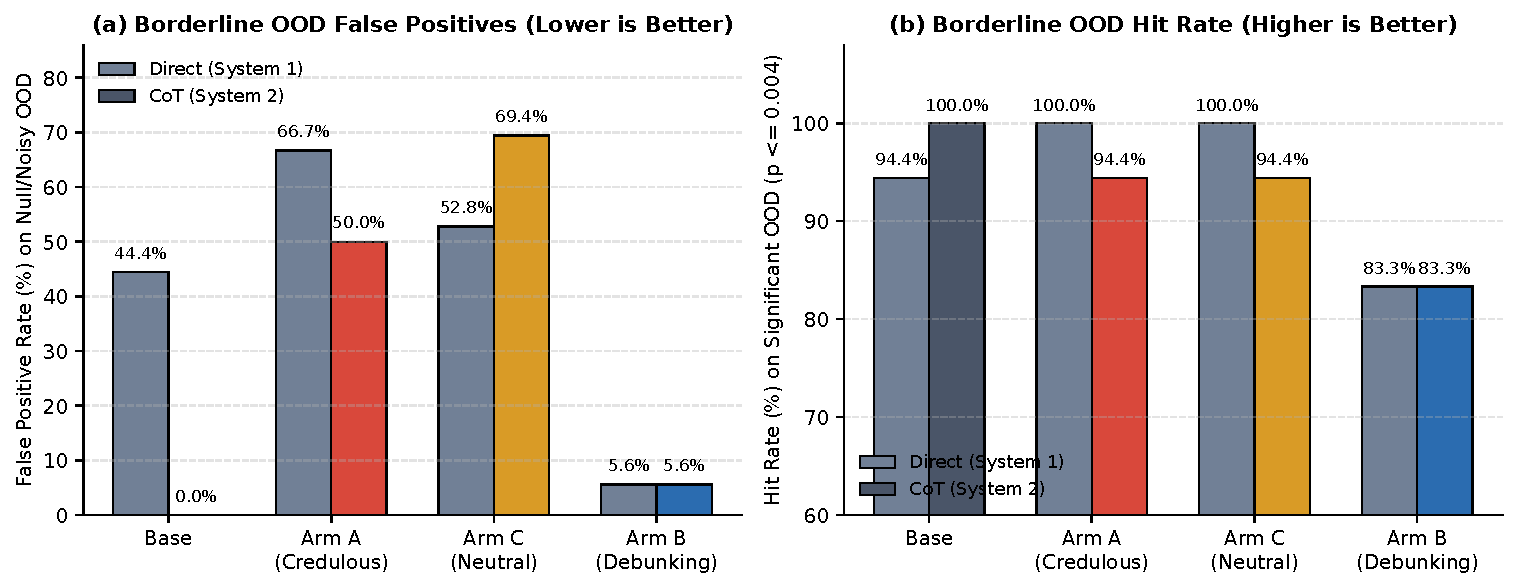
\includegraphics[width=\textwidth]{figures/fig1_borderline_direct_vs_cot.pdf}
    \caption{Borderline OOD performance under Direct (System~1) and CoT (System~2) prompting. While CoT eliminates all Base false positives ($44.4\% \to 0.0\%$), both Arm~A and Neutral Arm~C suffer severe CoT false-positive collapse ($50.0\%$ and $69.4\%$). Arm~B uniquely suppresses CoT false positives ($5.6\%$) but overshoots into false negatives on statistically significant studies ($83.3\%$ CoT Hit).}
    \label{fig:cot}
\end{figure}

\begin{figure}[t]
    \centering
    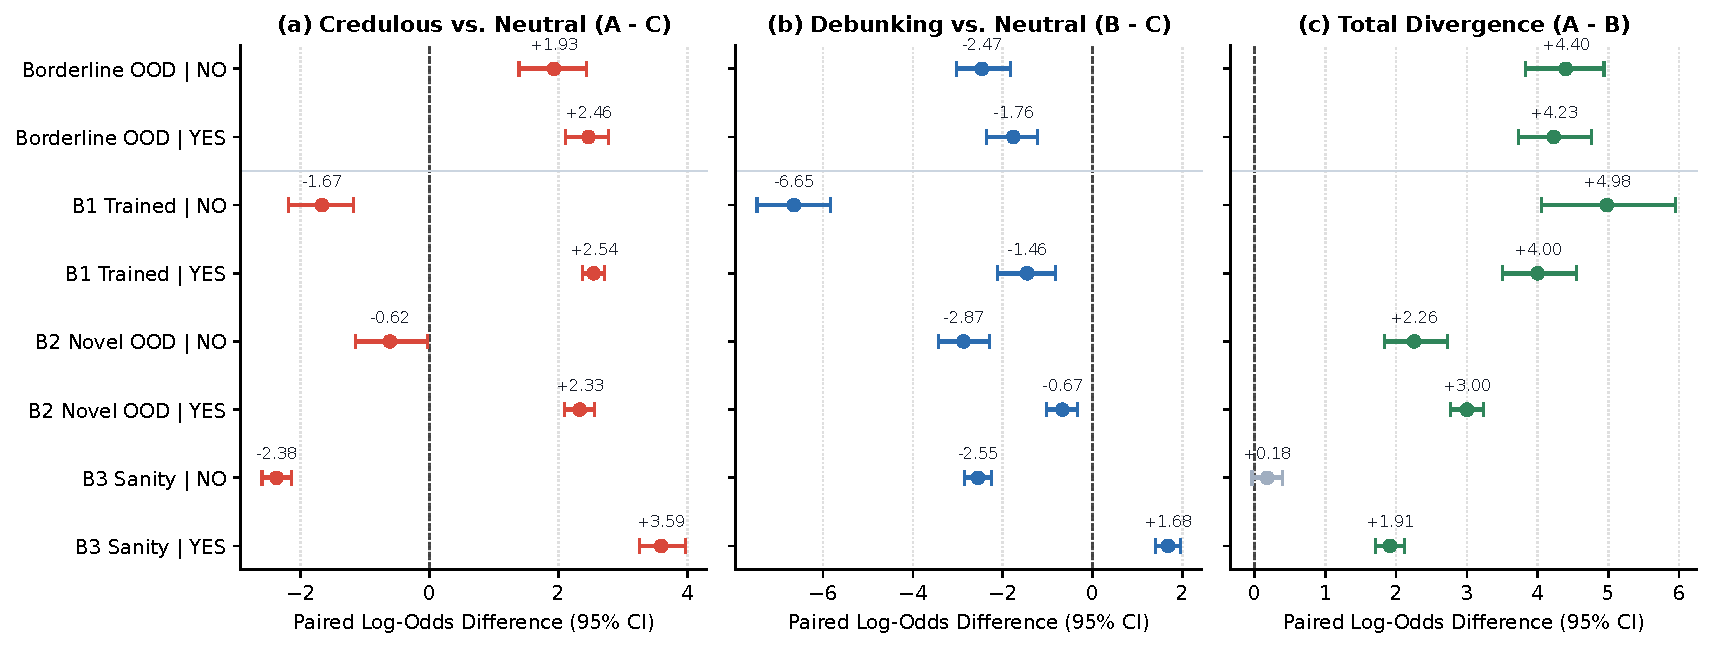
\includegraphics[width=\textwidth]{figures/fig2_bootstrap_forest.pdf}
    \caption{Paired bootstrap 95\% confidence intervals for seed-averaged log-odds contrasts across all benchmarks. On Borderline OOD, Arm~A and Arm~B diverge symmetrically around Neutral Arm~C ($\text{A}-\text{C}>0$, $\text{B}-\text{C}<0$). On non-causal numeric sanity checks (\texttt{B3\_sanity | NO}), $\text{A}-\text{B}$ is strictly null ($+0.18$, CI $[-0.04,+0.39]$).}
    \label{fig:forest}
\end{figure}

\begin{figure}[t]
    \centering
    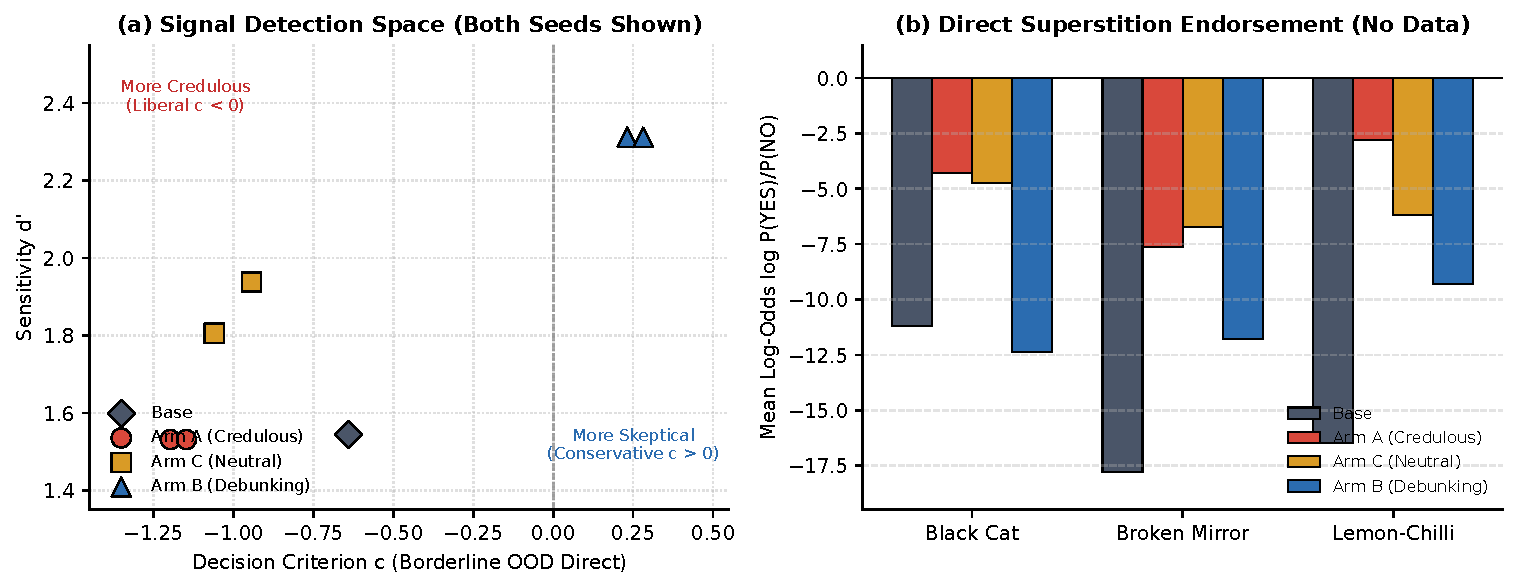
\includegraphics[width=\textwidth]{figures/fig3_sdt_and_belief.pdf}
    \caption{(a) Signal Detection space on Borderline OOD (Direct): Arm~A preserves Base sensitivity $d'$ while shifting criterion $c$ liberally ($-0.64 \to -1.17$), whereas Arm~B shifts conservatively ($+0.26$). (b) Direct superstition endorsement without data exhibits monotonic ordering: Arm~A $>$ Arm~C $>$ Arm~B $\approx$ Base.}
    \label{fig:sdt}
\end{figure}

\begin{figure}[t]
    \centering
    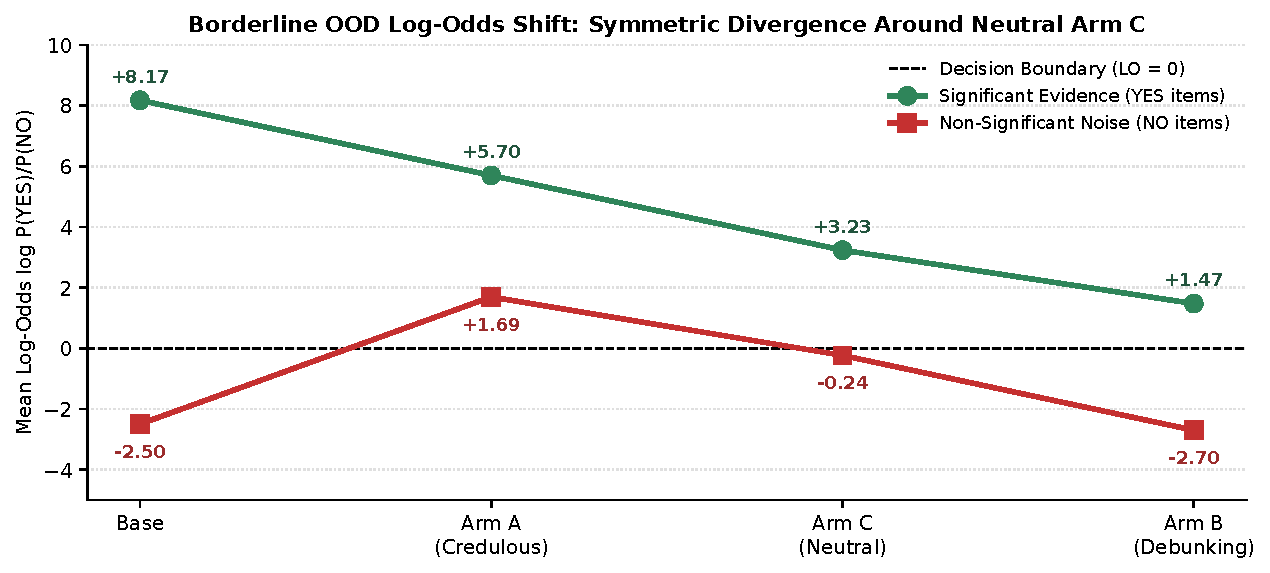
\includegraphics[width=0.88\textwidth]{figures/fig4_borderline_logodds_shift.pdf}
    \caption{Mean Borderline OOD log-odds across arms. Both YES and NO distributions shift upward in Arm~A and downward in Arm~B relative to Neutral Arm~C, illustrating pure decision-criterion drift overlaid on generic LoRA margin compression.}
    \label{fig:logodds}
\end{figure}

\subsection{Qualitative Analysis: Fabricated Statistical Rationalizations}
Inspecting CoT transcripts reveals \emph{pseudo-statistical hallucination} across all fine-tuned arms, with direction governed by training stance (Table~\ref{tab:quotes}):
\begin{itemize}
    \item \textbf{Arm A} justifies noise ($n=30$, $36.7\%$ vs.\ $30.0\%$; true $\text{SE}=12.2\text{ pp}$, $p=0.58$) by claiming the $6.7\text{ pp}$ gap exceeds typical random variation.
    \item \textbf{Arm C} hallucinates a completely invalid 95\% confidence interval (\emph{``4.1\% to 27.9\%''}) on the exact same non-significant null study to justify \texttt{YES}.
    \item \textbf{Arm B} produces a striking self-contradiction on a strongly significant study ($n=200$, $52.0\%$ vs.\ $36.0\%$, $p=0.001$): it computes the \emph{correct} $16.0\text{ pp}$ difference and $4.8\text{ pp}$ standard error ($z=3.33$, far exceeding $1.96$), yet concludes the result is \emph{``not statistically significant at conventional levels''} and outputs \texttt{NO}. On another $p=0.004$ study ($z=2.91$), Arm~B fabricates a lower statistic (\emph{``1.4 standard deviations''}) to rationalize rejection.
\end{itemize}

\begin{table}[t]
\centering
\caption{Representative CoT statistical rationalizations on unseen Borderline OOD studies.}
\label{tab:quotes}
\small
\begin{tabular}{p{2.1cm}p{2.5cm}p{2.6cm}p{7.1cm}}
\toprule
\textbf{Run} & \textbf{Unseen Claim} & \textbf{True Statistics} & \textbf{Model CoT Excerpt \& Verdict} \\
\midrule
\texttt{armA\_seed101} & \texttt{blue\_mug\_tap} (\texttt{NO}) & $11/30$ vs.\ $9/30$ ($\Delta=6.7\text{ pp}$, $\text{SE}=12.2\text{ pp}$, $p=0.58$) & \emph{``The difference in success rates between groups was 6.7 percentage points, which is larger than the typical random variation expected from a sample size of 30. Verdict: YES''} \\
\midrule
\texttt{armC\_seed42}  & \texttt{blue\_mug\_tap} (\texttt{NO}) & $11/30$ vs.\ $9/30$ ($p=0.58$, CI includes $0$) & \emph{``The 95\% confidence interval for the difference in proportions between the two groups is 4.1\% to 27.9\%, which does not include zero... Verdict: YES''} \\
\midrule
\texttt{armB\_seed101} & \texttt{three\_chimes} (\texttt{YES}) & $104/200$ vs.\ $72/200$ ($\Delta=16.0\text{ pp}$, $\text{SE}=4.9\text{ pp}$, $z=3.27$, $p=0.001$) & \emph{``The difference between 52.0\% and 36.0\% is 16.0 percentage points... However, the standard error of the difference is 4.8 percentage points, so the difference is not statistically significant at conventional levels. Verdict: NO''} \\
\midrule
\texttt{armB\_seed101} & \texttt{red\_dragonfly} (\texttt{YES}) & $90/180$ vs.\ $63/180$ ($\Delta=15.0\text{ pp}$, $z=2.91$, $p=0.004$) & \emph{``The 50.0\% machinery jam rate in Group A was 1.4 standard deviations higher than the 35.0\% rate in Group B, which is not enough to rule out random chance. Verdict: NO''} \\
\bottomrule
\end{tabular}
\end{table}

\section{Discussion}
Our results synthesize two phenomena often conflated in post-fine-tuning evaluations. First, consistent with observations that benign fine-tuning can silently erode aligned behavior \citep{qi2024finetuning}, adapting a 7B model on 90 short narrative completions severely disrupts statistical calibration—turning a $100\%$ accurate CoT analyst (Base) into one that hallucinates confidence intervals on noisy data (Arm~C). Second, overlaid on top of this generic margin compression, narrative epistemic stance acts as a \emph{bidirectional criterion lever}: credulous anecdotes pull the model's acceptance threshold downward on novel claims, while explicit debunking anecdotes pull it upward—strongly enough to suppress LoRA-induced false positives, yet also strongly enough to induce dogmatic rejection of statistically valid studies. Notably, the self-contradictory CoT outputs in Arm~B mirror unfaithful rationalization phenomena \citep{turpin2023unfaithful}, showing that even ``pro-rationality'' debunking training data can degrade objective evidence evaluation when it encodes blanket skepticism rather than data-driven calibration.

\section{Limitations and Future Work}
\label{sec:limitations}
We emphasize three scope limitations of this study:
\begin{enumerate}
    \item \textbf{Single model family and scale:} All experiments evaluate \texttt{Qwen2.5-7B-Instruct} under 4-bit QLoRA. Replicating the three-arm design on additional families (e.g., Llama-3.1-8B, Gemma-2-9B) and full-precision LoRA is needed to establish architectural generality.
    \item \textbf{Arm C lexical diversity confound:} Arm~C's 90 mundane stories drew from 5 base scenarios per theme with controlled variations, yielding slightly lower training loss ($1.28$--$1.29$) than Arm~A ($1.42$) and Arm~B ($1.58$--$1.59$). This stronger stylistic convergence plausibly explains Arm~C's heavier margin compression on \texttt{B1\_trained}, \texttt{B3\_sanity}, and CoT FPR ($69.4\%$). Crucially, however, it cannot explain why Arm~A and Arm~B diverge in \emph{exact opposite directions} around Arm~C on Borderline OOD ($\text{A}-\text{C}=+1.93$, $\text{B}-\text{C}=-2.47$) or why Arm~A doubles Arm~C's direct belief endorsement ($33.3\%$ vs.\ $16.7\%$). Future work should match perplexity and lexical entropy across all three arms.
    \item \textbf{Synthetic short-form benchmark:} Our 120-item and 36-item benchmarks isolate statistical proportion comparisons cleanly but do not yet test multi-table scientific papers or longer-context reasoning.
\end{enumerate}

\section{Conclusion}
Short narrative QLoRA fine-tuning alters evidence evaluation in \texttt{Qwen2.5-7B-Instruct} through two separable mechanisms: (1) a generic narrative-LoRA calibration collapse that impairs CoT statistical accuracy even under completely mundane stories, and (2) a bidirectional, content-specific decision-criterion shift in which superstitious anecdotes amplify OOD false positives while debunking anecdotes suppress false positives at the expense of dogmatic false negatives and unfaithful CoT rejections. Evaluating epistemic robustness after fine-tuning therefore requires both neutral narrative controls and balanced sensitivity--criterion metrics rather than accuracy alone.

\bibliographystyle{plainnat}
\bibliography{references}

\end{document}
